%%%
%%% Authors: Shahin, Tobia, Valerio
%%% TeX document for the presentation of the Biometric Systems Project
%%% @ Sapienza's Cyber-security Master Course.
%%%
\documentclass[t]{beamer}
\usecolortheme{beaver}

\usepackage[utf8]{inputenc}
\usepackage{wrapfig, float, graphicx}
\usepackage{csquotes}
\usepackage{hyperref}
\usepackage{beamerthemesimple}

\usepackage{tikz}
\usetikzlibrary{shapes.geometric,arrows,positioning,fit,calc}

\usepackage{listings} % Code inclusion
\lstset{
  basicstyle=\ttfamily,
  showstringspaces=false,
  commentstyle=\color{red},
  keywordstyle=\color{blue}
}

% Info to display in title page
\title
{
\LARGE Group Project
}
\subtitle
{
Biometric Systems
} 
\author[Casalino, Vendrame, Moghaddam] 
{
    Valerio Casalino (1916394)\inst{1} \and 
    Mario Tobia Vendrame (1922290)\inst{1} \and
    Shaahin Sabeti Moghaddam (1917507)\inst{1}    
}
\institute
{
\inst{1}
{\color{black} Cybersecurity Master @ Sapienza Università di Roma}
}
\date{
Fall 2019
}
\setwatermark{

\includegraphics[width=.4\textwidth]{img/logo}
}

\AtBeginSection[]
{
  \begin{frame}
    \frametitle{Table of Contents}
    \tableofcontents[currentsection]
  \end{frame}
}

\begin{document}
	
	\frame{\titlepage}

	\section{General Concepts \& Decisions}
	\begin{frame} \frametitle{Premise}

	Before we start, let us say that all of our work, included this own
	presentation, is open sourced and available on Github:
	
	\begin{center}
		\begin{figure}[H]
			
\includegraphics[width=.3\textwidth]{img/github}
		\end{figure}
		{\color{red} \url{https://github.com/casalinovalerio/biosys-project}}
	\end{center}
	\vfill
	There is also a script to replicate our setup for future projects.
	
\end{frame}

\begin{frame} \frametitle{Overview}
	We wanted a face recognition based authentication application that is simple, 
	yet particular. We deployed our test using:

	\vfill
	\begin{itemize}

		\item A \textbf{web interface} that works as a 
		demonstrative placeholder. It gets the face with the camera, makes 
		requests to our API server, which returns only a binary value for the 
		success of the authentication.
	
		\item An \textbf{API server}\footnote{Hosted by Digital Ocean: 
		{\color{red} \url{https://www.digitalocean.com/}}} that queries the 
		faces database and recognizes faces using the \textbf{@ageitgey's 
		tool}\footnote{Github project here: {\color{red} 
		\url{https://github.com/ageitgey/face_recognition}}}.
	
		\item A \textbf{database based on Blockchain}\footnote{Implemented by 
		Bigchaindb: {\color{red} \url{https://www.bigchaindb.com/}}} that is an
		open source wrapper for a blockchain database that can be queried with 
		standard SQL syntax. Implemented on the API server too.
	
	\end{itemize}
	\vfill
\end{frame}

\begin{frame} \frametitle{Overview scheme\footnote{Icons are licensed under 
	CC-BY 4.0. {\color{red} \url{https://fontawesome.com/license}}}}

	\begin{center} \begin{tikzpicture}
	
	\node[inner sep=0pt, label={above:casalinovalerio.com/biosys-project}] 
	(client) at (0,4) 
	{
\includegraphics[width=.11\textwidth]{img/laptop}};
	
	\node[inner sep=0pt, label={below:biosys.casalinovalerio.com}]
	(server) at (0,0) 
	{
\includegraphics[width=.11\textwidth]{img/server}};
	
	\node[inner sep=0pt, label={below:node1.casalinovalerio.com}]
	(database) at (6,0)
	{
\includegraphics[width=.09\textwidth]{img/database}};
	
	\draw[thick, ->] (client.south) -- node[anchor=west] {Request for auth}
	(server.north);
	\draw[thick, <->] (server.east) -- node[anchor=north] {query db} 
	(database.west);
	\draw[thick, ->] (server.west) .. controls (-2.5,2.5) .. 
	node[anchor=east] {Response} (client.west);
	
	\end{tikzpicture} \end{center}
	
\end{frame}	
	
	\section{Front-end Implementation}

	\section{Data-set Management}
	\begin{frame} \frametitle{The Block-chain database} 
	\begin{center}
		As database for new faces, we implemented a \textbf{Block-chain}. \\ 
		We used an open-source implementation of it, called 
		BigchainDB\footnote{Main page: {\color{red} 
		\url{https://www.bigchaindb.com}}. Documentation {\color{red}
		\href{http://docs.bigchaindb.com/projects/server/en/latest/introduction.html}
		{here}}.}. \\ We also used Docker\footnote{Main page: {\color{red} 
		\url{https://www.docker.com}}.} to deploy 4 containers running the
		application.
	\end{center}
	\vfill
	\begin{minipage}{.45\textwidth}
		\begin{figure}[H]
			
\includegraphics[width=.8\textwidth]{img/bchaindb}
		\end{figure}
	\end{minipage}
	\hfill
	\begin{minipage}{.45\textwidth}
		\begin{figure}[H]
			
\includegraphics[width=.8\textwidth]{img/dockerlogo}
		\end{figure}
	\end{minipage}
	\vfill
\end{frame}
	
\begin{frame} \frametitle{Architecture Implementation\footnote{This is absolutely not meant for a real deployment!!}}
	\begin{center} 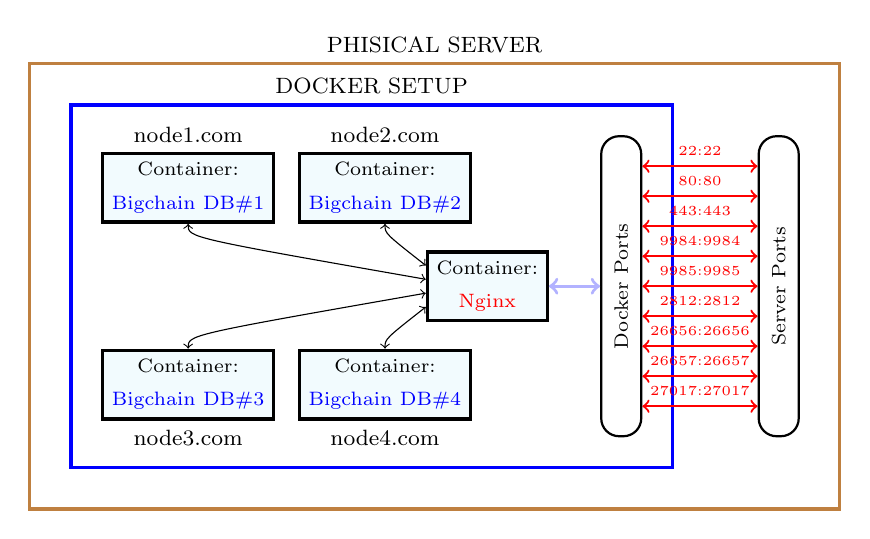
\begin{tikzpicture}[
		container/.style={rectangle, draw=black, fill=cyan!5 ,very thick, 
		minimum size=0.3in, align=center},
		ports/.style={draw=black, thick, rectangle, rounded corners=1.5ex,
		minimum height=0.2in, minimum width=1.5in,align=center, rotate=90}
	]
		
		% Bigchaindb dockers
		\node[container, label={above:\footnotesize node1.com}] 
		(1) at (1,3.5) 
		{\scriptsize Container: \\ \scriptsize \color{blue} Bigchain DB\#1};
		\node[container, label={above:\footnotesize node2.com}] 
		(2) at (3.5,3.5) 
		{\scriptsize Container: \\ \scriptsize \color{blue} Bigchain DB\#2};
		\node[container, label={below:\footnotesize node3.com}] 
		(3) at (1,1) 
		{\scriptsize Container: \\ \scriptsize \color{blue} Bigchain DB\#3};
		\node[container, label={below:\footnotesize node4.com}] 
		(4) at (3.5,1) 
		{\scriptsize Container: \\ \scriptsize \color{blue} Bigchain DB\#4};
		
		% Nginx container
		\node[container] 
		(5) at (4.8,2.25) {\scriptsize Container: \\ \scriptsize \color{red} Nginx};
			
		% Ports
		\node[ports] (6) at (6.5,2.25) {\scriptsize Docker Ports};
		\node[ports] (7) at (8.5,2.25) {\scriptsize Server Ports};
			
		% Outline Boxes	
		\node(n1)[draw, blue, very thick, fit=(1)(2)(3)(4)(5)(6), 
		inner sep=0.15in, label={above:\footnotesize DOCKER SETUP}]{};
		\node(n2)[draw, brown, very thick, fit=(n1)(7),
		inner sep=0.2in,label={above:\footnotesize PHISICAL SERVER}]{};
			
		% Containers to Nginx	
		\draw[<->] (1.south) .. controls + (down:0.5em) .. ([yshift=0.25em]5.west);
		\draw[<->] (2.south) .. controls + (down:0.35em) .. ([yshift=0.75em]5.west);
		\draw[<->] (3.north) .. controls + (up:0.5em) .. ([yshift=-0.25em]5.west);
		\draw[<->] (4.north) .. controls + (up:0.35em) .. ([yshift=-0.75em]5.west);
	
		% Nginx to docker ports			
		\draw[very thick,<->,blue!30] (5.east) -- (6.north);
				
		% docker ports to server ports	
		\draw[thick, red, <->] ([yshift=0.6in]6.south) -- 
		node[above]{\parbox[t]{2em}
		{\centering \tiny 22:22}} ([yshift=0.6in]7.north);
			
		\draw[thick, red, <->] ([yshift=0.45in]6.south) -- 
		node[above]{\parbox[t]{2em}
		{\centering \tiny 80:80}} ([yshift=0.45in]7.north);
		
		\draw[thick, red, <->] ([yshift=0.3in]6.south) -- 
		node[above]{\parbox[t]{3em}
		{\centering \tiny 443:443}} ([yshift=0.3in]7.north);
			
		\draw[thick, red, <->] ([yshift=0.15in]6.south) -- 
		node[above]{\parbox[t]{4em}
		{\centering \tiny 9984:9984}} ([yshift=0.15in]7.north);
	
		\draw[thick, red, <->] (6.south) -- 
		node[above]{\parbox[t]{4em}
		{\centering \tiny 9985:9985}} (7.north);
				
		\draw[thick, red, <->] ([yshift=-0.15in]6.south) -- 
		node[above]{\parbox[t]{4em}
		{\centering \tiny 2812:2812}} ([yshift=-0.15in]7.north);
				
		\draw[thick, red, <->] ([yshift=-0.3in]6.south) -- 
		node[above]{\parbox[t]{5em}
		{\centering \tiny 26656:26656}} ([yshift=-0.3in]7.north);
				
		\draw[thick, red, <->] ([yshift=-0.45in]6.south) -- 
		node[above]{\parbox[t]{5em}
		{\centering \tiny 26657:26657}} ([yshift=-0.45in]7.north);
			
		\draw[thick, red, <->] ([yshift=-0.6in]6.south) -- 
		node[above]{\parbox[t]{5em}
		{\centering \tiny 27017:27017}} ([yshift=-0.6in]7.north);
	\end{tikzpicture} \end{center}
\end{frame}
		
\begin{frame} \frametitle{How to interact with the DB}
	We are assuming that we have an enstablished connection set up.
	\vfill
	\begin{block}{Query data}
		\texttt{connection.searchAssets('AwesomeAsset') \\
		.then(assets =$>$ console.log('Found assets:', assets))\\
		// Read the console to look at the assets}
	\end{block}
	\vfill
	\begin{block}{Load data (make a transaction)}
		\texttt{// Create transaction first (txTransferBob)				
		driver.Transaction.signTransaction(txTransferBob, alice.privateKey);	
		\\conn.postTransactionCommit(txTransferBobSigned);}
	\end{block}
	\vfill
	Simple as that...
\end{frame}

	\section{APIs for Biometric Scanning Integration}
	
	\section{Performance Assessment}
	
	\section{Conclusions}


\end{document}
